\documentclass[conference]{IEEEtran}
%\IEEEoverridecommandlockouts
% The preceding line is only needed to identify funding in the first footnote. If that is unneeded, please comment it out.
%\usepackage{cite}
\usepackage{amsmath,amssymb,amsfonts}
\usepackage{algorithmic}
\usepackage{graphicx}
\usepackage{textcomp}
\def\BibTeX{{\rm B\kern-.05em{\sc i\kern-.025em b}\kern-.08em
    T\kern-.1667em\lower.7ex\hbox{E}\kern-.125emX}}
\usepackage{mathtools}

\usepackage[backend=biber]{biblatex}
\addbibresource{references.bib}

\DeclareMathOperator*{\argmin}{argmin}
\DeclareMathOperator{\E}{\mathbb{E}}
\newcommand{\norm}[1]{\left\lVert#1\right\rVert}

\renewcommand*{\bibfont}{\footnotesize}

\begin{document}

\title{Application of Stochastic Dynamic Programming to the Optimal Control of Hybrid Energy Storages in Electric Vehicles}

\author{\IEEEauthorblockN{Alok Deshpande}
\IEEEauthorblockA{University of Toronto - Energy Systems}
}

%\newenvironment{psmallmatrix}
%  {\left[\begin{smallmatrix}}
%  {\end{smallmatrix}\right]}

\maketitle

%\begin{abstract}
%This document is a model and instructions for \LaTeX.
%This and the IEEEtran.cls file define the components of your paper [title, text, heads, etc.]. *CRITICAL: Do Not Use Symbols, Special Characters, Footnotes, 
%or Math in Paper Title or Abstract.
%\end{abstract}

\section{Introduction}
Battery life is a factor that is critical for electric vehicle (EV) operation. It impacts vehicle performance in that an aging battery experiences a drop in energy capacity \cite{shi2017optimal}, which reduces the time between successive recharges and so the maximum distance that can be travelled on a single charging. Naturally, one would hope to maximize battery life.

In doing so, a common strategy being applied by vehicle designers is using a hybrid energy storage system, composed of a combination of a battery and a secondary energy storage operating in parallel \cite{thounthong2009energy}. (A common secondary storage device is a supercapacitor \cite{bambang2014energy}\cite{thounthong2009energy}\cite{7939849}, and so it will be referred to as such in this paper.) The reason is that the battery degrades when subject to fluctuating levels of energy demand (load) during the course of the trip. Experiments show that although it can store more energy (for example, 6-10 times higher density in a lead-acid battery \cite{bambang2014energy}), it should be operated with steady output power \cite{thounthong2009energy}. Discharging from the supercapacitor at times of fluctuating demand, then, allows one to improve battery life.

However, we cannot simply attempt to avoid cyclic loading of the battery; there are other factors that must be taken into account. For one, while the supercapacitor may normally be enough to satisfy the fluctuating demand (its lifetime under cyclic loading is about 1000 times longer \cite{thounthong2009energy}), the battery must still be used in cases of large fluctuations exceeding its limited capacity, such that the demand is always satisfied. Morevover, there is additional loss in transferring energy between devices, such that using a device out of its preferrable operating profile (e.g. cycling the battery) may be favourable under certain conditions. The complementary costs associated with each of these factors allow one to optimize the control of the hybrid battery-supercapacitor system. 

To optimally supply energy by controlling the storage devices, we employ  dynamic programming (DP). DP is well suited for optimal control in this situation because it can generate a control policy that is a function of the demand and can be administered at the rates at which demands arrive \cite{6183284}. It has previously been applied in the single battery case to determine the optimal amount of energy to charge and discharge (the control) so as to satisfy the demand \cite{su2013modeling}. We extend upon that model by adding the supercapacitor operating in parallel.

The DP approach requires that the state (energy) and control variables be both discretized in value and over time \cite{8330176}\cite{6254368}. For this application of DP, because precise control must be done with very small time steps to satisfy the fluctuating demand over a timespan of hours, an extremely large number of iterations would be involved if a finite horizon approach were chosen \cite{6183284}. From reviewing current literature applying DP to vehicular control contexts, we discovered that only \cite{8330176} and \cite{8315074} attempt to resolve this issue. We follow their approach of choosing an infinite horizon DP formulation, as we can safely approximate the number of steps to be infinite and assume that the energy transfer dynamics are time-invariant. More specifically, we apply value iteration (VI) to solve this DP, as \cite{8315074} does.

While a finite number of iterations is sufficient to approximate the steady-state solution to the infinite horizon DP \cite{Bertsekas:2007:DPO:1396348}, the DP still suffers from the curse of dimensionality when fine resolution in the control (i.e. high discretization) is required. To address this setback, we recognize that the exhaustive searches in the DP might be solved more quickly if the value iteration were reformulated as a linear program (LP), given the rapidity of current LP solvers. Uniquely, we reformulate the DP as an LP as per \cite{Bertsekas:2007:DPO:1396348} and others, and then use the result in \cite{4220813} to obtain the optimal control policy by solving its dual. Finally, we note that by eliminating certain infeasible states in this application, it is ultimately possible to reduce the computational complexity of the LP relative to the DP in some cases.

%its embedded exhaustive search taking very long

Hence, the novelty of this paper lies in:
\begin{enumerate}
    \item extending the black-box model in \cite{su2013modeling} to two storages,
    \item reformulating the DP as an LP where the demand is part of the state (uncontrollable component), and
    \item removing infeasible states to reduce the solution space of the LP.
\end{enumerate} The paper begins by modelling the problem in Section II and developing the infinite horizon DP in Section III. In Sections IV-V, the DP is reformulated as the dual LP. Finally, in Sections VI-VII, numerical results for the vehicle application are shown, and conclusions are drawn on the optimal response to various demand patterns. 

%Note that the DP and LP are compared both analytically and numerically to show the LP's relative computational benefits.


\section{Model}

\subsection{Definitions}
\begin{itemize}
	\item $t$: discrete time step index
	\item $h$: storage device number (1: battery, 2: supercapacitor)
	\item $\alpha^{C}$: charging efficiency\hspace{1em}
	$\alpha^{D}$: discharging efficiency
	\item $\beta$: storage efficiency factor
	\item $T$: number of steps (DP horizon)
	\item $K$: weighting for discharge cost relative to transfer loss
	\item $L$: energy demand (random)\hspace{1em}$E$: stored energy
	\item $D$: energy released by discharging
	\item $C$: energy consumed by charging
	\item $J$: value function
\end{itemize}

Let:
\begin{itemize}
	\item $W$ be the set of random perturbations, indexed by $1\leq k \leq M$
	\item $X$ be the set of states, indexed by $1\leq i \leq NM$
	\item $U$ be the set of controls, indexed by $1\leq p \leq P$
\end{itemize}

\subsection{Cost Function}
There are two relevant costs in this model:
\begin{enumerate}
    \item Discharge rate for the first storage device (battery):
	\begin{equation}K\left[D_{1}(t)\right]^{2}\end{equation}
	This objective is convex. A quadratic cost is chosen as referenced most commonly in literature \cite{bambang2014energy}, where it is used to penalize more for high excursions.
	\item Energy loss due to transfers:
	\begin{equation}
        (1-\alpha_{1}^{D})D_{1}(t)+(1-\alpha_{2}^{C})C_{2}(t)+(1-\alpha_{2}^{D})D_{2}(t)
	\end{equation}
	This objective is constrained to be non-negative. The energy transfers of charging ($C_{2}$) and discharging ($D_{1}$ and $D_{2}$) are arbitrarily chosen to be weighted by their inefficiencies ($1-\alpha$), as this penalizes the less efficient energy transfers.
\end{enumerate}

Hence, the sum of the objective functions (see below) is convex and non-negative.

\subsection{Optimization Problem}
Based on the above costs, the optimization problem is:

\begin{multline} \label{eq:initCostFnc}
    \min_{D_{1},D_{2},C_{2}}\Biggl[\sum_{t=0}^{T-1}
	(1-\alpha_{1}^{D})D_{1}(t)+
	(1-\alpha_{2}^{C})C_{2}(t)+\\
	(1-\alpha_{2}^{D})D_{2}(t)+
	K\left[D_{1}(t)\right]^{2}
	\Biggr]\end{multline}
subject to
\begin{itemize}
    \item Bounds on stored energy: 
	\begin{math}E_{h}^{min}\leq E_{h}(t)\leq E_{h}^{max}\end{math}
	\item Bounds on charging:
	\begin{math}0\leq C_{h}(t)\leq C_{h}^{max}\end{math}
	\item Bounds on discharging:
	\begin{math}0\leq D_{h}(t)\leq D_{h}^{max}\end{math}
	\item Energy balance:
	\begin{math}\left[D_{1}(t)\right] + \left[D_{2}(t) - C_{2}(t)\right] = L(t)\end{math}
\end{itemize}
and state equations $f_{1}(\cdot)$ and $f_{2}(\cdot)$ for the battery and supercapacitor, respectively:
\begin{itemize}
    \item \begin{math}E_{1}(t+1)=\beta_{1}E_{1}(t)-\frac{1}{\alpha_{1}^{D}}D_{1}(t)\end{math}
    \item \begin{math}E_{2}(t+1)=\beta_{2}E_{2}(t)+\alpha_{2}^{C}C_{2}(t)-\frac{1}{\alpha_{2}^{D}}D_{2}(t)\end{math}\newline
\end{itemize} Note that the energy balance equality constraint can be immediately substituted into the objective, which reduces the decision vector to $D:=(D_{1},D_{2})$. (More correctly, the minimization is done with respect to a vector $\textbf{D}$, whose components are $D(t)$ at $t=0,...,T-1$.  However, for the sake of clarity, we omit this formality.)

Critically, this paper chooses to take the expectation after the minimization. This is done so that the net energy discharged (control, $D$) exactly matches the demand, $L$, at all times and not its expected value, ensuring supply-demand balance.

In this model, $L(t)$ is a time-varying quantity which is observed at time t before a control $u(t):=(D_{1}(t),D_{2}(t))$ is applied, since the controller must have full knowledge of the demand before providing the control to satisfy it. Further, it evolves uncontrollably according to $L(t+1)=0L(t)+w(t)$, where $w(t)$ is a random variable which follows an unknown distribution and which represents a perturbation after the control is applied. Hence, we take $L(t)$ to be part of the state, $x(t):=(E_{1}(t),E_{2}(t),L(t))$. Doing so allows us to generate an optimal policy that a function of the load at time $t$, in addition to arbitrary energy state. (This choice of state makes the later LP formulation of this problem different from others reviewed in literature.)

With $x(t)$ being the state, the optimal value function \eqref{eq:initCostFnc} may be expressed in the general form:
\begin{equation}J^{*}[x(t)]=\mathop{\E}_{w(t)} \Biggl\{\min\left[\sum_{t=0}^{T-1}g(x(t),u(t),w(t))\right]\Biggr\}\end{equation}
where $g(\cdot)$ is called the stage cost. (Note that we avoid formality here, too, for brevity. Correctly, the expectation is with a respect to sequence of random variables whose terms are w(t) at $t=0,...,T-1$.) The value function can then be re-written in the form of Bellman's equation, which allows the problem to be solved by dynamic programming:
\begin{multline} \label{eq:FHDP}
J_{t}[x(t)]=\min g(x(t),u(t)) + \mathop{\E}_{w(t)} \{J_{t+1}[f(x(t),u(t),w(t))]\}
\end{multline}
where $f(\cdot)$ is a generalized function representing the transition equations $f_{1}(\cdot)$ and $f_{2}(\cdot)$.

Note that in this model, the random perturbation $w(t)$ that determines $L(t+1)$ depends on the energy in the subsequent state, $E(t+1):=(E_{1}(t+1),E_{2}(t+1))$. (This is because the demand at any iteration is limited to not exceed the total current energy at that iteration - i.e. we assume that vehicle will not be completely depleted of fuel.) However, the subsequent energy depends on the current energy through $f(\cdot)$, so in a manner respecting causality, the above expectation is more correctly conditioned on $x(t)$ and $u(t)$. While this conditioning is not shown, we do assume that $w(t)$ is Markovian.

\section{Infinite Horizon DP}
The above problem can be solved for $T$ control periods. However, for the very large values of T required in this application, the total cost $J$ will approach infinity, since each stage cost is non-negative. Thus, it is necessary to discount future costs by a factor $0<\alpha<1$.

With this modification, over multiple iterations the value function $J_{t}[x(t)]$ approaches the steady-state function $J(x)$. When a greedy policy is selected at each iteration, this function $J(x)$ is also optimal ($J^{*}(x)$). Hence, the infinite horizon problem is:
%(Theoretically, this is because the Bellman operation in \eqref{eq:FHDP} is a contraction mapping \cite{bertsekas1995dynamic}.)
\begin{multline} \label{eq:DP}
J^{*}(x)=\mathop{\E}_{w(t)} \Biggl\{\min\left[\sum_{t=0}^{\infty}\alpha^{t}g(x(t),u(t),w(t))\right]\Biggr\}
\end{multline}

When subject to the same constraints as \eqref{eq:initCostFnc}, this optimization problem is termed the infinite horizon DP formulation of optimal control for this paper. However, because we only use the infinite horizon approach for this application, henceforth we will simply use "DP" to refer to this infinite horizon DP.

It is common knowledge that a finite number of iterations is sufficient to allow $J_{t}[x(t)]$ to reach a steady-state value of $J^{*}(x)$ within a tolerance $\epsilon$. The method of solving these multiple iterations is called discounted value iteration with bounded cost per stage. In Section VII, we explain how we set this tolerance compared to that in the LP formulation. LP is now presented below.

%This DP program can be analyzed to determine its computational complexity. Firstly, with regards to the size of the problem, two matrices must hold data: the optimal cost, and the optimal control. By inspecting (6), it is clear that both the cost and control are functions of the state $(x,w)$, and so must have a size of $N\times M$. However, the previous costs must also be retained to determine that the costs are converging, so the required size is actually twice that (two matrices).

%The theoretical runtime can also be analyzed. Knowing that each iteration of DP involves nothing more than exhaustive searching (cost evaluation), and that $g(\cdot)$ is a function of the triplet $(x,u,w)$, the number of combinations to evaluate must be $NMP$. Over $k$ iterations, this is then $NMPk$ evaluations. According to theory \cite{Bertsekas:2007:DPO:1396348}, $k$ is related to the logarithm of the error tolerance on the constraints, and so it is also possible to estimate runtime in theory. However, this paper chooses to test the number of iterations from numerical examples, as detailed in Section 8.

%These computational characteristics for the DP will be compared to those of the LP, which is now presented below.


\section{Linear Programming formulation of DP}
Given that the value $J_{t}[x(t)]$ approaches an upper bound of $J^{*}(x)$ in VI, it is shown in \cite{Bertsekas:2007:DPO:1396348} how this means $J^{*}(x)$ can be calculated by solving a maximization problem. This is a linear programming problem whose optimal \textit{solution} is $J^{*}(x)$, rather than its optimal value as in VI. (Henceforth, the "costs" of the LP refer to possible solutions, and not the LP objective function values.)

%The expectation operator is linear, so this

In \cite{Bertsekas:2007:DPO:1396348}, Bertsekas presents an LP formulation of DP where the state has no uncontrollable components (in this case, the demand) that are randomly generated. We rewrite this in a form where the uncontrollable component is part of the state. Firstly, let:
\begin{itemize}
	\item $\lambda(x_{i})$ be the cost of state $x_{i}$ - i.e. $\boldsymbol{\lambda(x)}$ is a vector with the elements being costs in each state.
	\item $g(x_{i},u_{p})$ be the stage cost
	\item $p_{i,j}(u_{p})$ be the probability of moving from $x_{i}$ to $x_{j}$ by applying control $u_{p}$.
	%\item $Z$ be the set $Y\times U$
\end{itemize} Note that the subscripts are indices for vectors in the sets, and not indices of iteration.

Then, the probability $p_{i,j}(u)$ is defined as: \begin{align*} 
p_{i,j}(u_{p})&= P(x_{j}| x_{i},u_{p})\\ 
&= P(f(x_{i},u_{p},w_{k})| x_{i},u_{p})
\end{align*} The only random variable in the above expression is $w_{k}$, so we may express this instead as a probability of $w_{k}$:
\begin{align*} 
    p_{i,j}(u_{p})&= P(w_{k} | x_{i},u_{p})
\end{align*}

Hence, with the uncontrollable component now being a part of the state, the LP in \cite{Bertsekas:2007:DPO:1396348} can be expressed as:

\begin{equation} \label{eq:prelimLP}
\min_{\lambda(x_{i}) \forall i} \sum_{i=1}^{NM} -\lambda(x_{i})
\end{equation}

s.t. $\forall x_{i} \in X$: \begin{align*}
\lambda(x_{i})-\alpha\sum_{k=1}^{M}P(w_{k} | x_{i},u_{1})\lambda(f(x_{i},u_{1},w_{k})) &\leq g(y_{\textbf{i}},u_{1}) \\
&\vdots\\
\lambda(x_{i})-\alpha\sum_{k=1}^{M}P(w_{k} | x_{i},u_{P})\lambda(f(x_{i},u_{P},w_{k})) &\leq g(y_{\textbf{i}},u_{P})
\end{align*}

This is the LP to be solved to determine the solution to the DP. As a reminder, in the context of the hybrid storage problem, $x=(E_{1},E_{2},L)$ and $u=(D_{1},D_{2})$.

The problem can be expressed most succinctly in matrix form as:
\begin{equation} \label{eq:prelimLPmtx}
    \max_{\boldsymbol{\lambda}} \boldsymbol{1}^{T} \boldsymbol{\lambda}
    \hspace{1em}s.t.\hspace{1em}
    \boldsymbol{\lambda_{t}}-\alpha P\boldsymbol{\lambda_{t+1}} \leq \boldsymbol{g}
\end{equation} where:

\begin{itemize}
	\item $\boldsymbol{\lambda_{t}}$ is a vector containing P replicated vectors, $\boldsymbol{\lambda}$. Each vector $\boldsymbol{\lambda}$ contains the current state costs, $\lambda(x_{i})$, as its components. %Since each has size $NM\times 1$, the size of vector $\boldsymbol{\lambda_{t}}$ is $NMP\times 1$.
	
	\item $\boldsymbol{\lambda_{t+1}}$ also contains P replicated vectors, where each vector contains the costs for all next states $\lambda(x_{j})$. Importantly, $\boldsymbol{\lambda_{t+1}}$ belongs to the same state space as $\boldsymbol{\lambda_{t}}$. %Hence, the size of $\boldsymbol{\lambda_{t+1}}$ is also $NMP\times 1$.
	
	\item matrix $P$ is a block  matrix containing the conditional probabilities $p_{i,j}(u_{p})$. %The size of $P$ is $NMP\times NMP$.
	
	\item $\boldsymbol{g}$ contains the stage cost for each state-control pair. % , and current demand. The size of $\boldsymbol{g}$ is $NMP\times 1$
\end{itemize}

This form cannot yet be solved because there are two cost vectors. One may reduce this to a single decision vector by relating the next state cost to the current state cost.

Firstly, one can consider just the subset of costs associated with the $p^{th}$ control. This is done because each of the sets of linear inequalities in \eqref{eq:prelimLP} (i.e. all of the inequalities for fixed $p$) is of the same form, so the full matrix formulation will consist just of the concatenation of the individual matrix equations. For the $p^{th}$ control, the $p^{th}$ expression on the left in the set of linear inequalities of \eqref{eq:prelimLP} can be expressed in the form:

\begin{gather}\label{eq:mtxLPineq}
\begin{psmallmatrix}
& \lambda_{1}\\
& \vdots\\
& \\
& \lambda_{NM}
\end{psmallmatrix}
-
\alpha
\begin{psmallmatrix}
& P(w_{1}|x_{a}) \hdots  P(w_{M}|x_{a})  \\
P(w_{1}|x_{b}) \hdots  P(w_{M}|x_{b}) \\
\vdots\\
& P(w_{1}|x_{a}) \hdots  P(w_{M}|x_{a})  \\
& & \ddots
\end{psmallmatrix}
\lambda^{*}\end{gather} where $\lambda^{*} := \begin{psmallmatrix}
\lambda_{b+1} \hdots \lambda_{b+M} \lambda_{a+1}\hdots \lambda_{a+M} \hdots \end{psmallmatrix}^{T}$ is the vector of next state costs and the above matrix is an \textit{example} matrix of transition probabilities when the $p^{th}$ control is applied. Note that the notation $\lambda_{i}:=\lambda(x_{i})$ is used for brevity and that because this is specifically the $p^{th}$ expression, the conditional dependence on $u_{p}$ is suppressed.

Now, we consider the mapping between the current state and the next state to relate $\boldsymbol{\lambda_{t}}$ to $\boldsymbol{\lambda_{t+1}}$. Importantly, every triplet $(x_{i},u_{p},w_{k})$ leads to a next state $x_{j}=f(x_{i},u_{p},w_{k})$ that lies in the same set as the current state (set $X$). (Two possible current states associated with next states, $x_{a}$ and $x_{b}$, are shown to illustrate the form of P.) This implies that there exists a permutation mapping between the next state costs $\boldsymbol{\lambda_{t+1}}$ and the current state costs $\boldsymbol{\lambda_{t}}$. An example of a rearrangement equation could then take the following form:
\begin{gather} \label{eq:permMtx}
\lambda^{*}
=
\begin{psmallmatrix}
    \bold{0} & \hdots & \bold{0} & \bold{I} & \bold{0} & \hdots & \bold{0} \\
    \bold{0} & \bold{I} & \bold{0} & \bold{0} & \hdots & \hdots & \bold{0} \\
    & & & \vdots\\
\end{psmallmatrix}
\begin{psmallmatrix}
    & \lambda_{1}\\
    & \vdots\\
    & \\
    & \lambda_{NM}
\end{psmallmatrix}
\end{gather}

One can define $F$ to be the permutation matrix in \eqref{eq:permMtx}. Its actual form depends on the mapping between states (obtained from the state transition equations during offline optimization), but this illustrates the general structure.

Combining \eqref{eq:mtxLPineq} and \eqref{eq:permMtx}, the expression in the inequality of \eqref{eq:prelimLPmtx} can be expressed just in terms of a single decision variable. Hence, the LP in \eqref{eq:prelimLPmtx} can be re-written as:
\begin{equation} \label{eq:LPfinal}
    \max_{\boldsymbol{\lambda}} \boldsymbol{1}^{T} \boldsymbol{\lambda}
    \hspace{1em}s.t.\hspace{1em}
    (I-\alpha PF)\boldsymbol{\lambda_{t}} \leq \boldsymbol{g}
\end{equation}

This is the final form of the LP equivalent to the DP. %Note that based on the size of the matrix $F$, the size of $I-\alpha PF$ is $NMP\times NMP$.

\section{Dual LP Problem}
The above LP does not allow for directly determining the optimal policy upon convergence, so it is necessary to reformulate it as a minimization over some function of the optimal policy. This can be done by taking the dual of the LP, as shown in \cite{4220813}.

The dual of the LP can be expressed as:
\begin{equation}
    \max_{\boldsymbol{d}} -\boldsymbol{g}^{T} \boldsymbol{d}
    \hspace{1em}s.t.\hspace{1em}(I-\alpha PF)^{T}\boldsymbol{d} - \boldsymbol{1} = \boldsymbol{0}\hspace{1em}\boldsymbol{d} \geq \boldsymbol{0}
\end{equation}
where $\boldsymbol{d}$ is a vector of Lagrange multipliers for each state-control pair.

%the size of $\boldsymbol{d}$ is $NMP\times 1$.

Then, define $\pi$ to be the policy matrix, containing in its entries the probabilities of each action $u$ conditioned on state $x$. The policy for the optimal sequence, $\pi^{*}$, can be determined as follows, according to \cite{4220813}:

\begin{equation}
\pi^{*}(x,u)=\frac{d^{*}(x,u)}{\sum_{\forall u \in U}d^{*}(x,u)}
\end{equation} where $\boldsymbol{d^{*}}$ is the optimal solution to the dual LP.

Note that when the solution is searched on the vertices of the constraints, the matrix $\pi$ is purely deterministic \cite{MDPs}. This is to say it only contains binary entries, so the most optimal elements (control values at each state) are chosen with probability 1. Because a random control policy should be avoided, this means that the solution algorithm should only search on the vertices. For this reason, the simplex method is chosen for numerical simulation.

%At this point, the computational characteristics of this LP approach can also be investigated. The size of the program clearly consists of the size of the decision variables and the constraints. Firstly, by inspection, the size of the decision variable \boldsymbol{\lambda(y)} is $NM$ and the number of constraints (length of vector $\boldsymbol{g}$) is $NMP$. Additionally, the transition matrix $I-\alpha PF$ would account for most of the size of the problem, having a size of $NMP\times NMP$. However, it can be shown that the matrix $PF$ is quite sparse, given that $P$ and $F$ are. In practice, it was found from the results in Section 8 that the density can be very low (less than 1\%), so the problem size is approximately $NM + NMP$.

%As with DP, the computational time for the LP is partially dependent on the number of cost evaluations. $NMP$ evaluations must be done to determine the next state for each combination of control, to set up matrix F. Following this, however, K iterations of the (simplex) algorithm account for the rest of the time, where K is a function of M, N, and P. It has been shown empirically that the number of iterations is rarely more than three times the number of constraints \cite{bazaraa2010linear}, and certainly polynomial in $M,N,P$ \cite{doi:10.1287/moor.1110.0516}. This means $K\lessapprox3NMP$.

%By comparing these findings to those in Section 4, it can be seen that the LP has a larger size ($NM(P+1)$) than the DP ($3NM$). However, the number of cost evaluations is suggested to be lower in practice for the LP ($~4NMP$) compared to the DP ($kNMP$), using the same convergence tolerance for both methods. This suggests the LP method is empirically favoured when memory is not the major limitation, which is why it is chosen. Moreover, by removing so-called infeasible states in this particular application, the size of the LP can be even further reduced, as explained below.

Finally, by removing so-called infeasible states in this particular application, the size of the LP can be even further reduced. As explained below, this makes solving the LP a less computationally complex alternative to the DP.

\section{Numerical Solution}
To verify whether the above reasons favouring LP hold in practice, we perform a numerical test with data based on the energy storage application. Simulation is particularly important to be able to make a fair comparison between the two approaches because the number of iterations to solve the DP depends on the eigenvalues in the transition probability matrix \cite{Bertsekas:2007:DPO:1396348}, which are problem dependent. Moreover, in both approaches, the convergence time also depends on the error tolerance \cite{Bertsekas:2007:DPO:1396348}.

The critical aspect that needs to be considered when solving this optimal control numerically is the possibility for infeasible states. For this application, the inequality constraints that could be violated are those in \eqref{eq:initCostFnc}. In DP, one can see from \eqref{eq:DP} that the control is chosen from a subset $U(x_{i})$ so that the subsequent state in the minimization (given by $f(\cdot)$) is feasible. In practice, this just means that states with no feasible next state - for example, the state with no system energy and non-zero demand - are given an infinite cost in the minimization, which automatically forces the DP algorithm to avoid such states. Doing so implies that all possible next state costs are evaluated in DP when doing the minimization.

This technique is not possible for the LP in \eqref{eq:prelimLP} because the optimization is done over the costs themselves, so assigning a large cost will change the solution of the problem (and assigning an infinite cost will furthermore make the problem unbounded). (As a reminder, the "costs" in the LP refers to its decision variables, the components of $\boldsymbol{\lambda}$.) In this case, the approach we choose is to alter the problem setup by removing the infeasible states at the start. This also reduces the size of problem for two reasons. Firstly, the size of the decision vector $\boldsymbol{\lambda}$ decreases for fewer feasible states $x$ to which to assign a cost. Likewise, because the number of state costs that must be constrained is reduced, the number of constraints decreases. One can see how this would also decrease the computation time for the LP, as previously explained.

It is for this reason that we reformulate the original DP as an LP for this application. Unfortunately, it is not possible to derive the factors by which the size of the LP decreases in general, as they depend on the values of the problem parameters ($E^{max}$, etc.). In lieu of this, the numerical simulation is done with problems of different sizes to determine typical values for problem metrics (decision vector size and number of iterations). This also allows us to evaluate the optimal control policy when run online with various demand sequences. These results are discussed in the next section.


\section{Results}
In this paper, the optimization problems were solved numerically in MatLab for varying sizes of state space (cardinality $NM$) and $\epsilon$, with all other variables kept constant. Using constants $\alpha=0.99$, $\alpha_{C}=0.99$, $\alpha_{D}=0.9$, $\beta=0.99$, and $K=2$, the problems were solved to determine the optimal policy offline. Then, sample load sequences were applied to determine how the battery and supercapacitor should behave under different conditions with the policy. %The tests were run for 10 iterations, where each iteration involved determining the optimal control at a state and updating the state upon applying it.

Firstly, the DP problem was solved offline. It was tested online with three broad cases of demand: 1) constant, 2) ramp (continuously increasing/decreasing), and 3) fluctuating. Note that each sequence was randomly generated following a uniform distribution, for simplicity. Importantly, no excess demands were permitted based on the state (total energy stored), such that the conditional probabilities could still change over time as the state evolved.

In the case of a constant or ramp demand, it was determined that the battery will tend to supply the majority of the energy. Figures \ref{fig:ConstDemand} and \ref{fig:RampDemand} illustrate these two cases for one set of initial conditions.
\begin{figure}[htbp]
\centerline{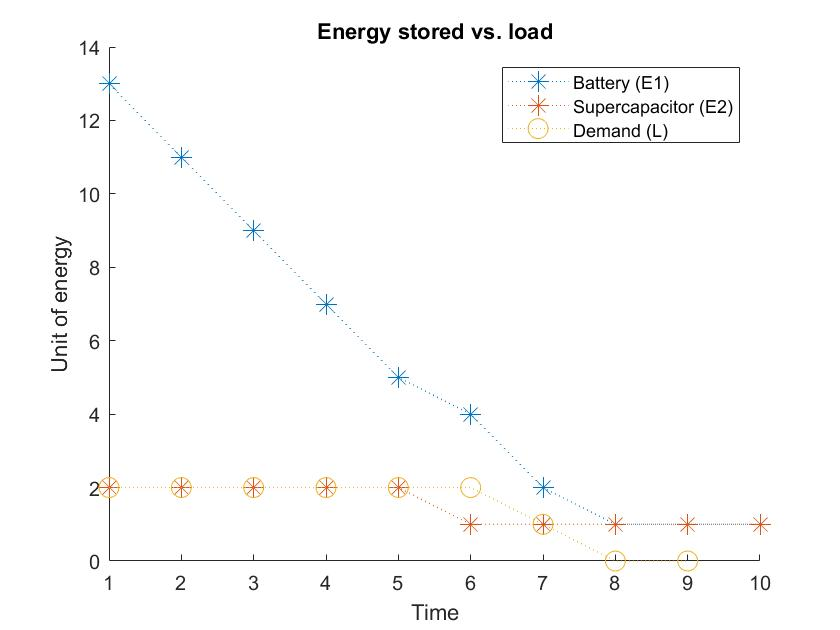
\includegraphics[width=3in,height=1.5in]{EnergyStoredvsload_ConstantLoad(E1_max=13,E2_max=2).jpg}}
\caption{Applying optimal policy from DP solution. Constant demand simulation, with N=$14\cdot3=42$, M=16.}
\label{fig:ConstDemand}
\end{figure}
\begin{figure}[htbp]
\centerline{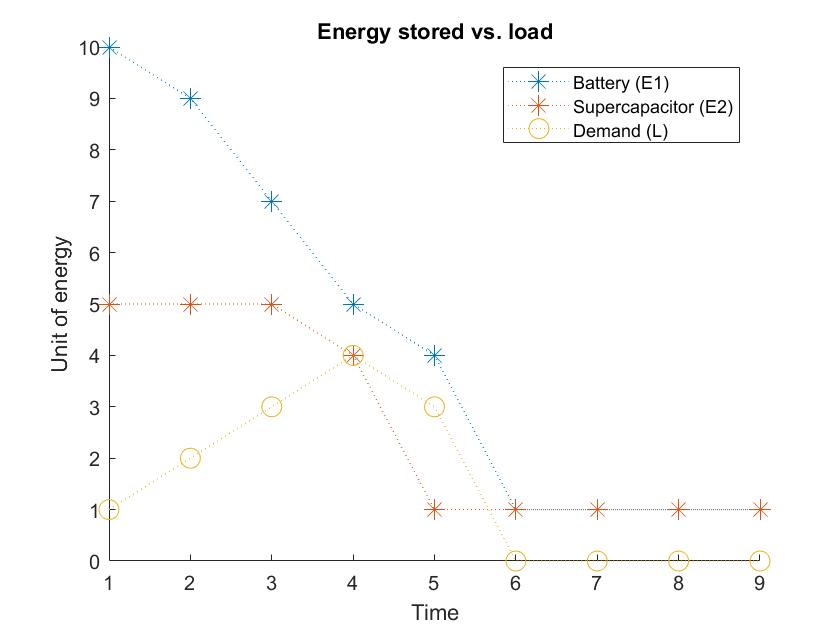
\includegraphics[width=3in,height=1.5in]{EnergyStoredvsload_RampLoad(E1_max=10,E2_max=5).jpg}}
\caption{Applying optimal policy from DP solution. Ramp demand simulation, with N=$11\cdot6=66$, M=16.}
\label{fig:RampDemand}
\end{figure} This result is expected because there is low cost for steady use of the battery (constant demand) or for limited cycling (ramp demand).

On the other hand, for fluctuating demand, the supercapacitor is used more, as illustrated in Figure \ref{fig:FluctuatingDemand}.
\begin{figure}[htbp]
\centerline{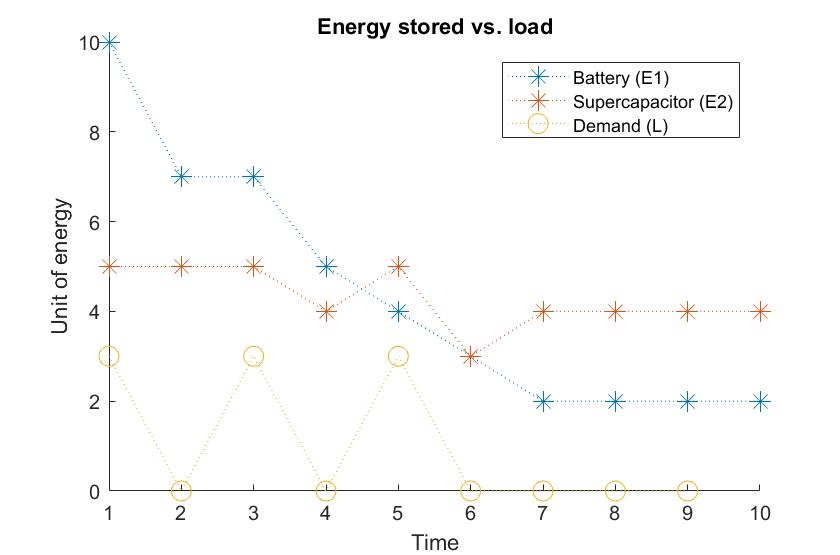
\includegraphics[width=3in,height=1.5in]{EnergyStoredvsFluctuatingLoad(E1=10,E2=5).jpg}}
\caption{Applying optimal policy from DP solution. Fluctuating demand simulation, with N=$11\cdot6=66$, M=16.}
\label{fig:FluctuatingDemand}
\end{figure} Clearly, the supercapacitor is now discharged at the start. However, this is still not as much use as expected. It was observed that by reducing the discharging efficiency of the battery, the supercapacitor is used more often (see Figure \ref{fig:FluctuatingDemand_LowBattEff}).
\begin{figure}[htbp]
\centerline{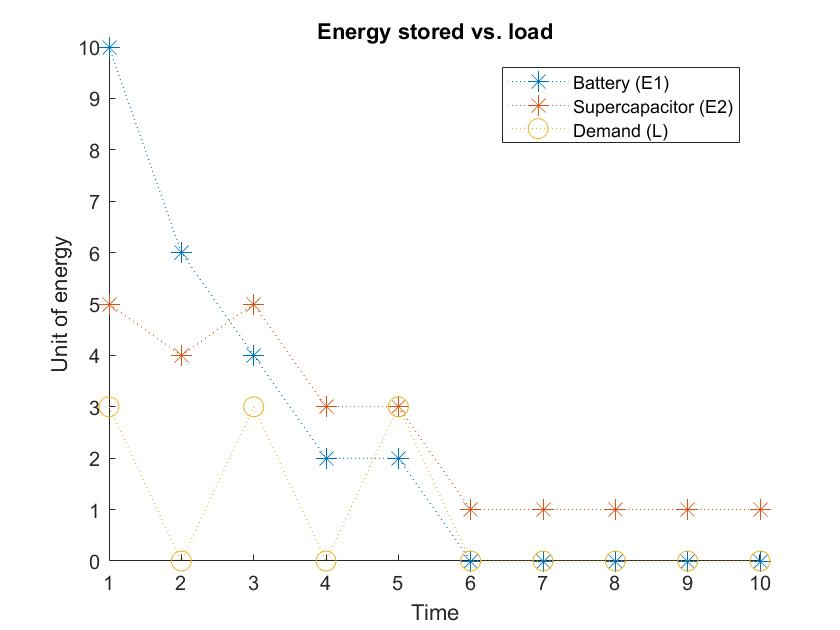
\includegraphics[width=3in,height=1.5in]{EnergyStoredvsFluctuatingLoad_LowBattEff(E1=10,E2=5).jpg}}
\caption{Applying optimal policy from DP solution. Fluctuating demand simulation, with N=$11\cdot6=66$, M=16. Lower battery efficiency (50\%).}
\label{fig:FluctuatingDemand_LowBattEff}
\end{figure} Hence, it is concluded that discharging the battery at the start of the sequence is still preferred because of the higher probability of large initial demands, unless the battery is inefficient.

One should also note how the battery is used to charge the supercapacitor, too. This can be seen, for example, in Figure 3 at time 4, where there is no demand but exchanges in the energy between the storage devices. This also confirms that the optimal policy makes forecasts, since a trade-off is made between instantaneous transfer loss and preempting satisfying future demands from a fully charged supercapacitor. Were it not for the benefits of the latter, there would be no reason for such energy exchanges.

Having characterized the policy obtained from solving the LP, the final step in establishing a computationally efficient and equivalent program for this application is to show that the LP gives the same results as the DP. As explained in Section V, the policy obtained using LP is the same as long as the primal yields the same optimal solution (costs). Hence, the error in costs obtained using either program needed to be quantified.

In this application, the value $J(x)$ is a 3-dimensional function of the state $x:=(E_{1},E_{2},L)$, and so would be stored as a 3D matrix of discrete states. We choose a metric for the error to be:
\begin{displaymath}
    e_{theor}=\frac{\norm{J^{*}_{DP}-J_{LP}}_{F}}{\norm{J_{LP}}_{F}}
\end{displaymath} where $\norm{\cdot}_{F}$ denotes the Frobenius norm, $J^{*}_{DP}$ is the optimal cost from solving the DP (equivalent to the true cost, $J^{*}$), and $J_{LP}$ is the optimal solution from solving the LP (possibly equal). $e_{theor}$ is the theoretical error if the value iteration had zero tolerance ($\epsilon=0$); in actuality, the value iteration solution ($J_{DP}$) approaches the true steady-state cost $J^{*}$ as $\epsilon$ decreases.
Moreover, we set the tolerance on satisfying the constraints of the LP ($\epsilon_{LP}=1e-9$) to be much lower than ($\epsilon$). For this reason, we assume that the LP has negligible error with respect to the true solution $J^{*}$ as long as the following error:
\begin{displaymath}
    e_{tot}=\frac{\norm{J_{DP}-J_{LP}}_{F}}{\norm{J_{LP}}_{F}}
\end{displaymath} monotonically decreases as $\epsilon$ decreases. In such a case, it is known that the LP leads to an equal solution as the DP. Table \ref{tab:Table1} shows results indicating that this is indeed the case.
\begin{table}%[htbp]
	\begin{center}
		\begin{tabular}{|c|c|c|}
			\hline
			\textbf{VI Convergence Tolerance ($\epsilon)$}&\textbf{Iterations}&\textbf{$e_{tot}$} \\
			\hline
			1e-3& 5 & 0.824\% \\
			\hline
			1e-4& 12 & 0.0423\% \\
			\hline
			1e-6& 1100 & 0.0188\% \\
			\hline
		\end{tabular}
	\end{center}
	\caption{Decrease in total error of LP relative to DP as the DP tolerance is decreased}
	\label{tab:Table1}
\end{table} Therefore, this result empirically supports the claim that the LP is equivalent to the DP.

Finally, in addition to quantifying the error for LP, the LP is also compared to DP based on computational complexity. Table II provides simulation results for the number of iterations as the model size and tolerances (of \textit{both} programs) are varied.

\begin{table}[htbp]
	\begin{center}
		\begin{tabular}{|c|c|c|c|}
			\hline
			\textbf{Size of}&\textbf{Tolerances}&\multicolumn{2}{|c|}{\textbf{Number of Iterations}} \\
			\cline{3-4} 
			\textbf{Problem} & \textbf{$(\epsilon=\epsilon_{LP})$} & \textbf{DP} &  \textbf{LP} \\
			\hline
			N=30, M=10& 1e-3 & 5 & 15 \\
			\hline
			N=30, M=10& 1e-4 & 12 & 17 \\
			\hline
			N=66, M=16& 1e-3 & 44 & 38 \\
			\hline
			N=66, M=16& 1e-4 & 52 & 47 \\
			\hline
		\end{tabular}
	\end{center}
	\label{tab:Table2}
	\caption{Comparison of DP and LP algorithm times when optimizing the two-storage model}
\end{table} The experimental results in this table show that LP generally takes longer to converge for small problems, but is faster for large problems. Hence, this suggests that the LP formulation may be a more efficient program for this two-storage application.

%While the size of problems and number of cost evaluations were compared in Sections 4 and 6 for the general case, the number of iterations very application-dependent, as previously explained.

\section{Conclusion}
In conclusion, this paper has developed and optimized a model for energy transfers from two parallel storage devices satisfy a random demand. The model is an extension of the case with a single storage device, and was formulated using dynamic programming. Its optimal control policy can be applied to exactly satisfy a real-time demand, making it suitable for applications such as EVs.

To better meet the timescales and computational limits associated with this application, the DP was modified in two steps. Firstly, value iteration was used to solve the DP as an infinite horizon DP, which allowed for determining the optimal controls with long application times. Additionally, the DP was reformulated as an equivalent LP, with benefits coming in reducing the computational time. %at the expense of more memory use.

Lastly, the final program was simulated with three classes of demand to determine the optimal control in each case. As expected, it was found that high-energy or steady demands lead to more use of the battery, whereas fluctuating demand leads to more use of the complementary storage device. This means the policy produced by the program should work to reduce battery degradation, based on literature reviewed.

The final simulation results confirmed that the final LP is indeed a more efficient algorithm in terms of reducing time. However, further work remains to be done to scale the problem to the energies expected in a real application, where minimizing over the large number of states remains a challenge.

\printbibliography

\end{document}